\graphicspath{{images/}}

\section{Methods}
\label{sec:methods}

\subsection{CANS}

To analyse QFA data using the competition model I developed the Python
package CANS which can be used for model composition, model
simulation, parameter inference, and visualisation of results. CANS
accepts cell density timecourses for any size rectangular array. CANS
can produce SBML models to document results of parameter inference or
for independent validation using other simulation tools. It is
relatively simple to create and simulate new models involving
reactions between species within cultures or between neighbouring
cultures, and to fit these provided an initial guess. The CANS package
is available at
\href{https://github.com/lwlss/CANS}{https://github.com/lwlss/CANS}.


% \subsection{\thesubsection~Description of datasets}

\subsection{The P15 dataset}
\label{sec:P15_description}

I compared logistic and competition model performance by fitting both
models to QFA data for a single plate, ``P15''
(Figure~\ref{fig:p15_section}), from a study by
\citet{Addinall2011}. P15 is a 384-culture QFA plate using deletions
from plate-15, a standard deletion library in \textit{S. Cerevisiae},
with background mutation \textit{cdc13-1}. \textit{cdc13-1} is a
temperature dependent conditional mutatation in a gene involved in
telomere stability. Internal cultures consist of 6 repeats of each of
49 different strains with a deletion in a second gene thought to be
relevant to telomere function. There are also 14 repeats of a strain
with a neutral deletion, \textit{his3}\(\Delta\). Edge cultures are
also inoculated with repeats of \textit{his3}\(\Delta\), but estimates
from these cultures are discarded due to noise in cell density
estimates caused by reflections from plate walls. Cultures were
inoculated with \(\sim\)100 cells which is below levels of
detection. P15 was incubated at 27\(^{\circ}\)C, where
\textit{cdc13-1} starts to experience loss of function. Each culture
has cell density estimates taken at 10 timepoints over 4 days. I
elected to study P15 because of the large variation in fitness between
strains, which may induce competition effects. There are also many
repeats of each strain with which to calculate
statistics. Furthermore, independent validation data from spot tests
exists in published studies for several strains
\citep{maringele2002exo1,zubko2004exo1,Holstein20141259,foster2006mrx}.

\subsection{The Stripes and Filled plate datasets}
\label{sec:stripes_description}

The Stripes and Filled plates (Figure~\ref{fig:stripes_images}) are
from a QFA experiment designed to study competition (personal
communications E. Holstein (April 2016)). On the Stripes plate
(Figure~\ref{fig:stripes_images}a), strains are inoculated in every
other column, leaving gaps. As for P15
(Section~\ref{sec:P15_description}), strains have a background
mutation \textit{cdc13-1} and a deletion in a second gene. There are
more strains than for P15 and most cultures have no repeats. The same
strains as in the Stripes plate were inoculated in the same positions
on the Filled plate (Figure~\ref{fig:stripes_images}b). These were
inoculated from the same liquid culture to try to reduce variation. In
the Filled plate, gaps are now filled with new cultures. Each deletion
in a new column is a transposition of the strain immediately to the
left but with a different background mutation,
\textit{rad75}\(\Delta\). The left most column is filled with the same
neutral deletion, \textit{his3}\(\Delta\). The new strains with
\textit{rad75}\(\Delta\) are generally fitter than the common strains
with \textit{cdc13-1}. A higher inoculum denstiy (\(\sim\)10,000
cells) was used compared to P15 and this was detectable at time
zero. Both plates were incubated at 27\(^{\circ}\)C, where
\textit{cdc13-1} starts to experience loss of function, and
photographed at \(\sim\)50 timepoints over 4 days: around five times
more often than for P15.

The experiment is designed to exhibit differences in growth between
the same strains on each plate; cultures on the Stripes plate should
have access to more nutrients because they grow next to empty
locations; cultures on the Filled plate should have access to less
nutrients and experience more competition due to the extra
neighbours. I used the QFA data from both plates for cross-plate
calibration and validation of the competition model by simulating
timecourses for the Stripes plate using parameters estimated by
fitting the Filled plate.

\subsection{Solving and fitting}

\subsubsection{Solving}
\label{sec:solving_comp}
% [Only keep if I remove the CANS overview above: To analyse QFA data I
% created a Python package (``CANS'') for model composition, model
% simulation, parameter inference, and visualisation of results. CANS
% accepts timecourse data of cell density for any size rectangulare
% array.]\\

CANS numerically solves models using one of two methods. The first is
slower and uses SciPy's integrate.odeint to solve models written in
Python at user supplied timepoints. I vectorised code using NumPy to
optimise solving of the competition model by this method. For solving
a plate of 384 cultures with cell density observations at 10 unevenly
spaced time points, I found that solving time decreased from tenths to
hundredths of a second (10 times faster) using the Python bindings for
libRoadRunner. libRoadRunner requires models to be written in SBML so
I wrote code using the libSBML Python API to automatically generate
SBML versions of the competition model for any size plate.
% //I could go into more detail about how models are defined// but
% maybe this is not needed.
Unlike SciPy's odeint, libRoadRunner only simulates at uniformly
spaced timepoints. To fit QFA cell observations, which are not made at
fixed time intervals, requires simulated cell amounts at the observed
timepoints. For the analysis of P15, where each timecourse has only 10
timepoints, I simulated sequentially between pairs of timepoints. This
method was slower for the analysis of the Stripes and Filled plates
where each timecourse had around 50 timepoints. To increase speed, I
used SciPy's interpolate.splrep to make a 5th order B-spline of cell
density timecourses with smoothing condition \(s=1.0\). I evaluated
the spline for cell density using SciPy's interpolate.splev at 15
evenly spaced timepoints from time zero to the time of the last QFA
observation. I then solved these timecourses with one call to
RoadRunner.simulate.

When using RoadRunner on a modern CPU, fitting a full plate with 10
unevenly spaced timepoints takes \(\sim\)3 hours; fitting a full
plate using a spline with 15 timepoints takes \(\sim\)1 hour.
\\\\

% Fitting
\subsubsection{Fitting the competition model}
\label{sec:fitting_comp}

I use QFA data after processing with Colonyzer \citep{Lawless2010}.
Colonyzer uses integrated optical density measurements in whole plate
images as a proxy for cell density. I used timecourse cell density
estimates, which have arbitrary units, throughout my analysis. I fit
the competition model using a gradient method and made maximum
likelihood estimates of parameters using a normal model of measurement
error. For constrained minimisation I used the L-BFGS-B algorithm from
SciPy's integrate package.

I determined stopping criteria so that parameters of full-plate
simulated data sets, with a small amount of simulated noise, were
recovered with high precision. To help the minimizer, I scaled
\(C(0)\) values by a factor of \(10^{5}\) to make parameter values
closer in order of magnitude. I ran repeated fits using different
parameter guesses for each plate (see Sections~\ref{sec:P15_fit} and
\ref{sec:cross_plate_val_results}). I set bounds according to
Table~\ref{tab:p15_bounds} and checked that best fits had no
parameters at a boundary.
%
\begin{center}
  \captionof{table}{\textbf{Parameter bounds.} Used for fitting the
    competition model to P15 and the Stripes and Filled plates. Bounds
    on \(N(0)\) were applied to both \(N_{I}(0)\) and \(N_{E}(0)\) for
    internal and edge cultures. ``guess'' refers to the initial guess
    of each parameter (see Section~\ref{sec:initial_guess}).}
  \begin{tabular}{| c | c c |}
    \hline
    Parameter        & Lower Bound  & Upper Bound \\
    \hline
    \(C(0)\)     & guess x \(10^{-3}\)  & guess x \(10^{3}\)\\
    \(N(0)\)     & guess / \(2\)  & guess x \(2\)\\
    % \(N^{I}(0)\) \& \(N^{E}(0)\) & guess / \(2\)  & guess x \(2\)\\\\
    \(k\)        & 0.0    & 10.0\\
    % \(b\) (all cultures)           & 0.0    & \(\infty\) \\
    \(b\)           & 0.0    & None \\
    \hline
  \end{tabular}
  \label{tab:p15_bounds}
\end{center}
%
%%%% Boundary conditions Two N_0 %%%%%
Cultures at the edge of a plate have an advantage because they have
access to a greater area of nutrients. I corrected for this using a
separate parameter \(N^{E}(0)\) representing a higher initial amount
of nutrients in edge cultures. In rate equations involving edge
cultures, I scaled edge culture nutrient amount \(N_{i}\) by the ratio
\(N^{I}(0)/N^{E}(0)\), where \(N^{I}(0)\) is the amount of nutrients
in internal cultures. The physical interpretation of this correction
is that edge cultures have an extra supply of nutrients that can
diffuse instantly into the reaction volume. This treatment reduced the
error in cell density estimates for cultures one row or column inside
the edge and resulted in better fits to internal cultures overall (see
Table~\ref{tab:corner} in
Section~\ref{sec:treatment_of_boundaries}).

Cell density measurements from edge cultures contain more noise due to
reflections from plate walls \citep{Lawless2010}. For the competition
model, I collectively fit to all cultures and selected best fits based
on only the fit to internal cultures.

% %%%% Empties %%%%%
% (Can go to results section or Stripes method section:) QFA data for
% the Stripes plate contained observations for cultures that were known
% to be empty. When fitting the competition model, I set growth constant
% \(b\) to zero for these cultures and removed them from fitting.
%%%% End Empties %%%%%

\subsubsection{Fitting the logistic model}

Fitting the mass action logistic model requires using culture level
\(N(0)\) and creating 383 extra parameters. The QFA R package
\citep{qfa2016} can fit the standard logistic model and has heuristic
checks to correct a confounding of parameters that occurs when
slow-growing cultures are dominated by noise. I did not have time to
implement these checks for the mass action logistic model, so I
instead fit using the QFA R package. This is not equivalent because
QFA R does not fit data collectively and instead uses a culture level
\(C(0)\) (1152 total parameters). However, this is a useful comparison
with a method of analysis previously used in QFA, including for the
analysis of P15 \citep{Addinall2011}. I do not expect much
disagreement of fitness estimates with the mass action logistic model
once heuristic checks are implemented. In contrast to the competition
model, noisy data from edge cultures can be discarded before fitting.
% I conduct model comparison between the competition and logistic
% models in sections (Results sections).

\subsubsection{Data visualisation}

I created plotting functions in CANS to visualise fits and simulations
of QFA timecourses and to compare the ranking of fitness estimates
using the Python package matplotlib.

\subsection{Parameter conversion}
\label{sec:parameter_conversion}

When \(k\) is set to zero, the competition model
(\ref{eq:competition_model}) reduces to the mass action logistic model
which has the same sigmoidal solution as the standard logistic
model. In this limit, it is possible to equate C species of both
models and convert parameters using,
% Derivation or link to blog.
\begin{subequations}
  \label{eq:conversion}
  \begin{align}
    &r_{i} = b_{i}(C(0) + N(0)),\\
    &K = C(0) + N(0).
    % &r = b(C(0) + N(0))\\
    % &K = (C(0) + N(0))
  \end{align}
\end{subequations}
%
The reaction equation of the competition model (\ref{eq:reaction})
assumes that all nutrients are converted to cells. This implies that
all cultures starting with the same amount of nutrients reach the same
final amount of cells. Therefore, to fit the mass action logistic
model to QFA data, it is necessary to allow \(N(0)\) to vary for each
culture which is not physically realistic and, in which case, the mass
action logistic model has the same number of parameters (769) as the
standard logistic model.
%
Figure~\ref{fig:correction} shows fits of a single culture on a larger
16x24 format plate using both models. This culture grew faster than
its neighbours (not shown) and, according to the competition model,
competed for more nutrients.
%
Figure~\ref{fig:correction}a shows the mass action logistic model fit
where \(N(0)\) is estimated as being approximately equal to the final
cell amount, or equivalently, carrying capacity \(K\).
%
Figure~\ref{fig:correction}b shows the competition model fit with a
plate level \(N(0)\) and \(k > 0\). Re-simulating with \(k\)
set to zero gives the dashed mass action logistic model curves which
are corrected for competition. We can therefore obtain the corrected
logistic model \(r_{i}\) and \(K_{i}\) of these curves by converting
from competition model estimates of \(b_{i}\), \(C(0)\), and
\(N(0)\). N.B. \(b\) is the same for both the solid and dashed
curves in Figure~\ref{fig:correction}b.

% This produces the correction in \(r\) and \(K\) between the two fits
% (see Figures~\ref{fig:correction}) and allows direct comparison
% between competition and logistic model estimates.
%

Competition model \(C(0)\) and \(N(0)\) are the same for all cultures
on a plate. Therefore, by the conversion equations
(\ref{eq:conversion}), all cultures on a plate have the same carrying
capacity \(K\) and all \(b_{i} \propto r_{i}\) by the same
factor. Similarly, \(MDP\) is the same for all cultures and all
\(b_{i} \propto MDR_{i}\) by the same factor (see
Equation~\ref{eq:MDR_MDP}). Therefore, \(b\) is equivalent to common
QFA fitness measures, \(r\), \(MDR\), and \(MDR*MDP\) (see
e.g. \citet{Addinall2011}). This makes \(b\) a very convenient fitness
measure for the competition model; we need not convert to logistic
model parameters to compare the fitness rankings of cultures on the
same plate. To compare competition model fitness rankings between
different plates we can of course use \(b\). However, this is not
equivalent to comparing \(r\) or \(MDR\) as different plates may have
different \(C(0)\) and \(N(0)\).

\begin{Figure}
  \centering
  \graphicspath{{images/correction/}}
  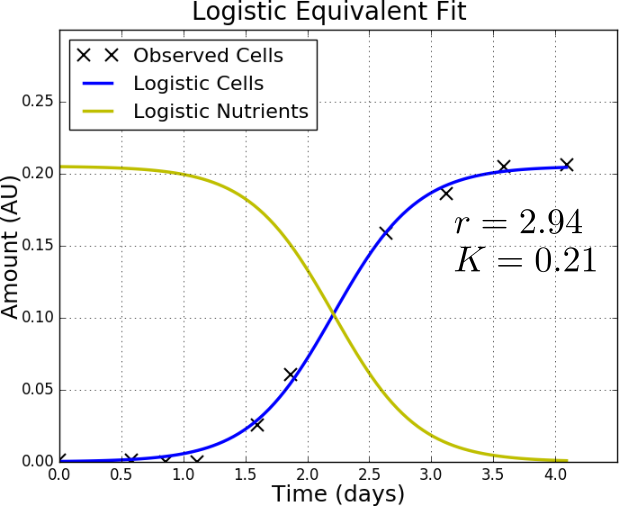
\includegraphics[width=\linewidth]{final/logistic}
  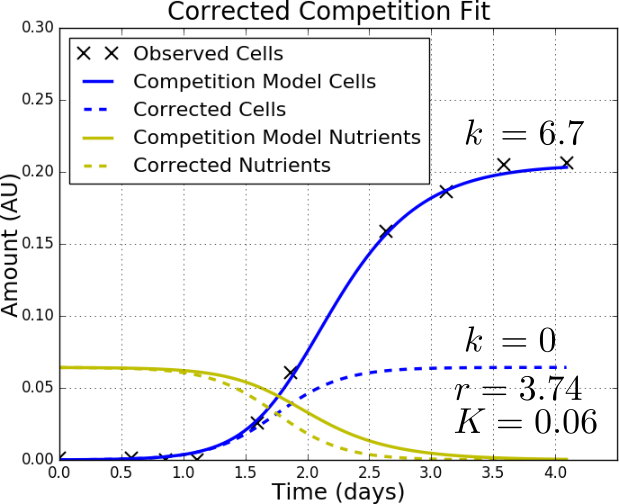
\includegraphics[width=\linewidth]{final/competition}
  \captionof{figure}{\textbf{Using the competition model to correct
      for competition.} Fits are to culture (R10, C3) of P15 which
    grew faster and reached a higher final cell density than its
    neighbours (not shown). According to the competition model, this
    is because this culture competed for more nutrients. To reach the
    same final cell density, the mass action logistic model requires a
    higher amount of starting nutrients for this culture and a
    different amount for each neighbour. The correction to the
    competition model simulates how growth would have appeared without
    competition and, for the culture shown,
    gives~\(r_{corrected} >
    r_{logistic}\)~and~\(K_{corrected} < K_{logistic}\).}
  \label{fig:correction}
\end{Figure}

\subsection{Determining initial parameters}
\label{sec:initial_guess}

Collectively fitting the competition model to a standard 384-format
QFA plate is a formidable optimisation problem involving 384
timecourses and 387 parameters. Achieving good fits therefore requires
making a good initial guess. To fit small simulated zones I could
simply use many random parameter guesses. However, for a full plate
the chance of any random guess being close to the ``true'' values
diminishes and more sophisticated guessing methods are required. I
developed the \textit{Imaginary Neighbour Model}
(Figure~\ref{fig:imag_neigh_schematic}) for guessing competition model
\(b_{i}\) and this allowed good fits of to be made. As the project
progressed, it became clear how to convert between fast logistic
parameter estimates and competition model parameters (see
Section~\ref{sec:parameter_conversion}) and this could be a valid
alternative.

\subsubsection{Guessing initial amounts}
\label{sec:guessing_amounts}

Recall from the competition model reaction equations
(\ref{eq:reaction} and \ref{eq:diffusion_reaction}) that nutrients can
only diffuse or be converted to cells. Thus, assuming that reactions
are nearly complete at the end of cell observations and that
\(C(0) \ll C(\infty)\), the total initial amount of nutrients,
\(N_{Tot}\), can be estimated using,
\begin{equation}
  \label{eq:N_Tot}
  N_{Tot} = n_{I}N_{I}(0) + n_{E}N_{E}(0) \approx C_{F},
\end{equation}
where \(C_{F}\) is the total of final cell measurements, \(n_{I}\) and
\(n_{E}\) are the numbers of internal and edge cultures, and
\(N_{I}(0)\) and \(N_{E}(0)\) are initial nutrient amounts
for internal and edge cultures (see
Section~\ref{sec:fitting_comp}). Using (\ref{eq:N_Tot}), and an estimate
for the ratio of area associated with edge cultures to area associated
with internal cultures,
\(A_{r} = A_{E} / A_{I} = N_{E}(0) / N_{I}(0)\), I made
guesses of \(N_{I}(0)\) and \(N_{E}(0)\) using,
%
\begin{equation}
  \label{eq:N_0_guesses}
  \begin{aligned}
    % &A_{r} = A_{E} / A_{I} = N_{E}(0) / N_{I}(0)\\
    % &N_{Tot} = n_{I}N_{I}(0) + n_{E}N_{E}(0) \approx C_{F}\\
    &N_{I}(0) = N_{Tot} / (n_{I} + n_{E}A_{r})\\
    &N_{E}(0) = N_{Tot} / (n_{I}/A_{r} + n_{E}).
    % &N_{E}(0) = (N_{Tot} - n_{I}N_{I}(0)) / n_{E}.
  \end{aligned}
\end{equation}
%
When \(A_{r} = 1\), (\ref{eq:N_0_guesses}) reduces to the initial
nutrient guess for the one initial nutrient parameter model. I used
\(A_{r} = 1.5\).

In QFA using dilute cultures, \(C(0)\) falls below the level of
detection. I did not estimate initial guesses of \(C(0)\) and instead
ran multiple fits over a range of \(C(0)\) values in logspace chosen
to encompass uncertainty in \(C(0)\) for the given experiment. I
expressed this as a ratio, \(C_{r}\), multiplied by the initial
nutrient guess \(N(0)_{I}\).

% ; for P15 \(10^{-5}\) to \(10^{-3}\) times the
% average final cell amount, for the Stripes and Filled plates
% \(10^{-7}\) to \(10^{-1}\) times average final cell amount.


\subsubsection{\boldmath Guessing \(b\) \unboldmath}
\label{sec:guessing_b}
%%%%%%%%%%%%%%% Imag neigh %%%%%%%%%%%%%%%%%%%

\graphicspath{{images/imag_neigh_schematic/}}
\begin{Figure}
  \centering
  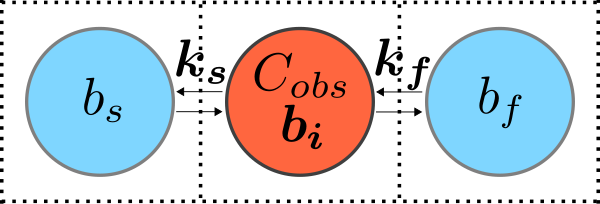
\includegraphics[width=\linewidth]{final/imag_neigh_schematic_2}
  \captionof{figure}{\textbf{Schematic of the imaginary neighbour
      model.} I developed this model to make quick guesses of
    competition model \(b_{i}\) by fitting single cultures. A real
    culture (red) with cell observations, \(C_{obs}\), is modelled as
    growing alongside imagined slow and fast growing neighbours (blue)
    with growth constants \(b_{s}\) and \(b_{f}\) (for slow and
    fast). The model uses separate nutrient diffusion constants
    \(k_{s}\) and \(k_{f}\) for slow and fast growing neighbours
    rather than a single parameter \(k\). \(k_{s}\), \(k_{f}\), and
    the growth constant \(b_{i}\) of the real culture are estimated by
    fitting the model to \(C_{obs}\) with all other parameters
    fixed. Different numbers of each neighbour can be chosen to
    replicate different configurations of neighbours that might be
    present on a real plate.}
  \label{fig:imag_neigh_schematic}
\end{Figure}

% The model aims to approximate the diffusion of nutrients into and out
% of a culture using an configuration of imagined fast and slow growing
% neighbours. Cell observations for a culture can be fit to get
% estimates of growth constants \(b_{i}\).\\

To guess competition model \(b_{i}\) I used the imaginary neighbour
model (Figure~\ref{fig:imag_neigh_schematic}) to quickly fit
individual cultures. The model is based on the reaction and rate
equations of the competition
model~(\ref{eq:reaction}--\ref{eq:diffusion_reaction}) but tries to
replicate the diffusion of nutrients into and out of a culture using
imaginary fast and slow growing neighbours, with growth constants
\(b_{f}\) and \(b_{s}\), and different nutrient diffusion constants
\(k_{f}\) and \(k_{s}\). To fit the model to QFA data, I fixed
\(C(0)\) and \(N(0)\) for all cultures by the initial guesses (see
Section~\ref{sec:guessing_amounts}), I fixed \(b_{f}\) at a high value
and fixed \(b_{s} = 0\), I allowed \(b\), \(k_{f}\), and \(k_{s}\) to
vary with lower bound zero and no upper bound. I used initial values
of zero for \(k_{f}\) and \(k_{s}\). I carried out multiple fits of
the imaginary neighbour model for each value of \(C_{0}\), with
initial values for \(b\) taken from the range (35, 40, ..., 100) and
\(b_{f}\) fixed as 1.5 times this value. I determined the number,
\(n\), of each neighbour from the guess of \(N_{I}(0)\) and the range
of final cell amounts, such that the culture with the highest observed
final cell density had enough slow growing neighbours to provide all
of the nutrients necessary to reach this final cell density. I solved
the imaginary neighbour model using SciPy's odeint and fit using a
gradient method as in Section~\ref{sec:fitting_comp}. Fits of the
imaginary neighbour model take several minutes which is fast compared
to fits of the competition model which take on the order of hours.

%%%%%%%%%%%%%%% Imag neigh %%%%%%%%%%%%%%%%%%%%%%%%%%%%%%%%%%%%%%

\subsubsection{\boldmath Guessing \(k\) \unboldmath}

Simulations of the competition model using sets of \(b\) parameters
drawn from different normal distributions have linear relationships
between variance in final cell amount and nutrient diffusion constant
\(k\). I simulated guessed parameters \(C(0)\), \(N(0)\), and
\(b_{i}\) with a range of different \(k\) values and used linear
regression to parameterise the straight line. I then took the variance
in final cell amount for real data and used the regression model to
predict \(k\).
% \\\\
% Don't think I need this figure. r->b and make titles bigger. Fitted
% \(k\) was much higher so I should probably resimulate over a
% bigger range. Only possibly to know in hindsight. I could also use the
% fitted parameters for this rather than drawing from a normal
% distribution.
% \\
% \graphicspath{{images/guessing/}}
% \begin{Figure}
%   \centering
%   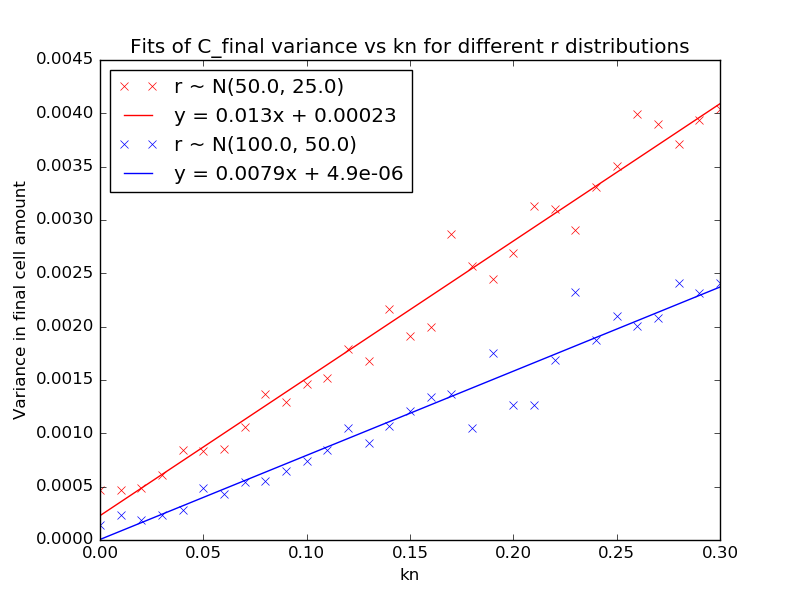
\includegraphics[width=\linewidth]{final/kn_guessing}
%   \captionof{figure}{\textbf{Guessing \(\bm{k}\) from the variance in
%       final cell amounts.} The competition model is simulated for a
%     16x24 format plate using two random sets of culture-level \(b\)
%     parameters drawn from different normal distributions. Each set of
%     \(b\) parameters is simulated with a range of \(k_n\) parameter
%     values. The variance in final cell density for all cultures is
%     plotted against \(k_n\) for each simulation. Lines are shown for
%     least squares fits to points from each set of \(b\) parameters.}
%   \label{fig:kn_guessing}
% \end{Figure}

% \subsection{\thesubsection~Development of a genetic algorithm}

% I began work on a hierarchical genetic algorithm method of parameter
% inference inspired by the hierarchical Bayesian analysis of QFA data
% by \citet{Heydari2016}. (I'm not sure that it is too similar or was in
% fact inspired by this.)

% p15 cell ratios
% cell_ratios = np.logspace(-3, -5, num=5)

% stripes and filled cell ratios
% cell_ratios = np.logspace(-1, -7, num=10) I increased the range to
% account for higher inoculum density and work of Herrmann.
%
% Results \(C(0)\), \(N_{I}(0)\), \(N_{E}(0)\), \(k\)
% est_params Stripes [ 0.00831517,  0.08524787,  0.09564223,  1.92525936]
% est_params Filled [ 0.00617039,  0.11660628,  0.1830217 ,  4.84354755]


%%% Local Variables:
%%% mode: latex
%%% TeX-master: "report"
%%% End:
